\chapter{Methodology}
\label{ch:method}

This chapter describes the design and implementation of MedPrepAI within the clinical-lab repository. We formalize the platform architecture, document each major subsystem, and explain LLM integration, persistence, and access governance.

\section{System Overview}
MedPrepAI is a three-tier web application:
\begin{itemize}
  \item \textbf{Presentation tier}: Next.js 15 (React, TypeScript, Tailwind CSS, Radix UI) with server and client components, API routes for LLM proxying, and role-based navigation (\texttt{menu.config.ts}).
  \item \textbf{Application tier}: NestJS 10 REST API with Swagger, JWT auth, guards, scheduled jobs, and Socket.IO realtime module.
  \item \textbf{Data tier}: MySQL 8 with Prisma ORM using a \textbf{multi-file schema} (\texttt{backend/prisma/schema/*.schema.prisma}) merged via \texttt{schema.prisma}.
\end{itemize}

We model the platform as:
\begin{equation}
\mathcal{S} = \langle \mathcal{U}, \mathcal{A}, \mathcal{D}, \mathcal{L}, \mathcal{G}, \mathcal{R} \rangle
\end{equation}
where $\mathcal{U}$ is the set of user-facing applications (student dashboard, faculty workspace, landing, payments), $\mathcal{A}$ is the API surface (Nest modules), $\mathcal{D}$ is the persistence layer (Prisma models), $\mathcal{L}$ is the LLM orchestration layer (Gemini via frontend API routes and backend services), $\mathcal{G}$ is the governance layer (RBAC, subscriptions, entitlements), and $\mathcal{R}$ is realtime infrastructure (notifications, chat, websockets).

Each clinical encounter session $s$ in MedPrep AI is:
\begin{equation}
s = \langle u, m, c, \Sigma, M, \omega \rangle
\end{equation}
with user $u$, mode $m \in \{\textsc{Practice}, \textsc{Learning}, \textsc{Evaluation}, \textsc{Shadow}\}$, case $c$, message transcript $\Sigma$, auxiliary artifacts $\omega$ (SOAP, diagnosis, hints), and status $M$ (ACTIVE, COMPLETED, ABANDONED), persisted as \texttt{MedprepConversation}.

Figure~\ref{fig:architecture} illustrates the high-level architecture. Figure~\ref{fig:module-groups} groups backend modules by domain.

\begin{figure}[htbp]
  \centering
  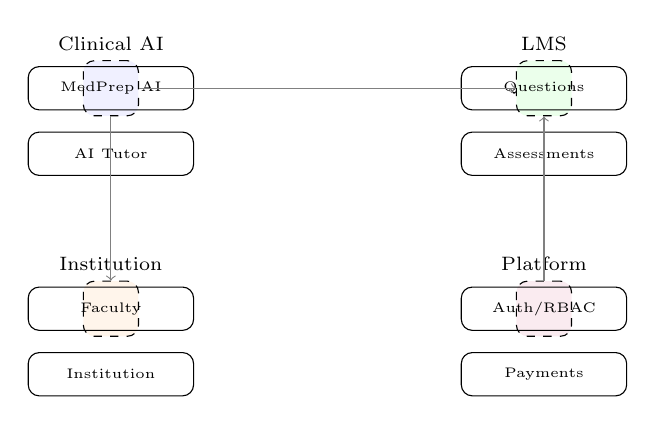
\begin{tikzpicture}[
    mod/.style={rectangle, draw, rounded corners, minimum width=2.1cm, minimum height=0.55cm, font=\tiny, align=center},
    grp/.style={rectangle, draw, dashed, rounded corners, inner sep=0.35cm}
  ]
    \node[grp, fill=blue!6, label={[font=\scriptsize]above:Clinical AI}] (g1) at (0,0) {};
    \node[mod] at (g1) {MedPrep AI};
    \node[mod, below=0.55cm] at (g1) {AI Tutor};
    \node[grp, fill=green!8, label={[font=\scriptsize]above:LMS}] (g2) at (5.5,0) {};
    \node[mod] at (g2) {Questions};
    \node[mod, below=0.55cm] at (g2) {Assessments};
    \node[grp, fill=orange!8, label={[font=\scriptsize]above:Institution}] (g3) at (0,-2.8) {};
    \node[mod] at (g3) {Faculty};
    \node[mod, below=0.55cm] at (g3) {Institution};
    \node[grp, fill=purple!8, label={[font=\scriptsize]above:Platform}] (g4) at (5.5,-2.8) {};
    \node[mod] at (g4) {Auth/RBAC};
    \node[mod, below=0.55cm] at (g4) {Payments};
    \draw[->, gray] (g1) -- (g2);
    \draw[->, gray] (g1) -- (g3);
    \draw[->, gray] (g4) -- (g2);
  \end{tikzpicture}
  \caption{NestJS module groups in MedPrepAI backend (logical layering).}
  \label{fig:module-groups}
\end{figure}


\begin{figure}[htbp]
  \centering
  \begin{tikzpicture}[
    node distance=0.9cm and 1.2cm,
    box/.style={rectangle, draw, rounded corners, minimum width=2.6cm, minimum height=0.75cm, align=center, font=\small},
    layer/.style={rectangle, draw, dashed, inner sep=0.35cm}
  ]
    \node[box] (web) {Next.js Frontend\\Pages + Components};
    \node[box, right=of web] (api) {Next API Routes\\LLM Proxy};
    \node[box, below=of web] (nest) {NestJS Backend\\Modules + Guards};
    \node[box, right=of nest] (gemini) {Google Gemini};
    \node[box, below=of nest] (db) {MySQL + Prisma};
    \node[box, right=of db] (stripe) {Stripe Payments};
    \draw[->] (web) -- (api);
    \draw[->] (web) -- node[right,font=\scriptsize]{REST/JWT} (nest);
    \draw[->] (api) -- (gemini);
    \draw[->] (nest) -- (db);
    \draw[->] (nest) -- (stripe);
    \draw[->] (nest) -- (gemini);
  \end{tikzpicture}
  \caption{High-level architecture of MedPrepAI (clinical-lab).}
  \label{fig:architecture}
\end{figure}

\section{Technology Stack}
Table~\ref{tab:stack} summarizes core technologies.

\begin{table}[htbp]
  \centering
  \caption{Technology stack of MedPrepAI.}
  \label{tab:stack}
  \begin{tabular}{@{}ll@{}}
    \toprule
    \textbf{Layer} & \textbf{Technologies} \\
    \midrule
    Frontend & Next.js 15, React, TypeScript, Tailwind, Radix, TanStack Table, Stripe.js \\
    Backend & NestJS, Passport JWT, Swagger, Socket.IO, @nestjs/schedule \\
    Database & MySQL, Prisma 5 (multi-schema), migrations, seed scripts \\
    AI & @google/generative-ai (Gemini 2.5 Flash default) \\
    Auth & bcrypt passwords, JWT, token blacklist guard \\
    Payments & Stripe (subscriptions, invoices, wallets) \\
    Deploy & PM2, Nginx reverse proxy, AWS EC2 (documented) \\
    \bottomrule
  \end{tabular}
\end{table}

\section{Database Design}
The Prisma schema partitions concerns across files:
\begin{itemize}
  \item \texttt{base.schema.prisma}: Users, roles, permissions, audit logs, institutions.
  \item \texttt{content.schema.prisma} / \texttt{product.schema.prisma}: LMS hierarchy and products.
  \item \texttt{assessment.schema.prisma}: Question papers and attempts.
  \item \texttt{subscription.schema.prisma}: Packages, features, entitlements.
  \item \texttt{medprep.schema.prisma}: Conversations, messages, SOAP, diagnosis, hints.
  \item \texttt{faculty.schema.prisma}, \texttt{student.schema.prisma}: Assignments and activity.
  \item \texttt{chat.schema.prisma}, \texttt{notification.schema.prisma}: Collaboration.
  \item \texttt{ai-tutor.schema.prisma}, \texttt{mock-exam.schema.prisma}, \texttt{achievement.schema.prisma}, etc.
\end{itemize}
Indexing supports hot paths (e.g., \texttt{@@index([userId, mode, status])} on conversations). JSON metadata columns store case snapshots and shadow-mode intervention payloads without schema churn.

\section{Authentication, RBAC, and Entitlements}
\subsection{JWT Authentication}
Users authenticate via \texttt{POST /auth/login}; the backend issues JWTs embedding \texttt{userId}, \texttt{email}, \texttt{roles}, and \texttt{permissions}. A token blacklist service supports logout invalidation (\texttt{JwtAuthWithBlacklistGuard}).

\subsection{Role-Based Access Control}
Roles include Admin, Student, and InstitutionManager (extended with Faculty profiles). Decorators (\texttt{@Roles}, \texttt{@Permissions}) combine with \texttt{RolesGuard} and \texttt{PermissionsGuard}. The frontend mirrors checks via \texttt{useAccessControl} and \texttt{ProtectedRoute}.

\subsection{Subscription Features and MedPrep Mode Gating}
\texttt{SubscriptionsService} resolves active packages and features (Qbank, Self Assessment, Study Planner, MedPrep modes). \texttt{MedprepAiService.assertMedprepModeAllowed} maps subscription slugs (\texttt{let-me-drive}, \texttt{qa}, \texttt{ai-evaluation}, \texttt{shadow-mode}) to enum modes. Distinct-case quotas prevent abuse of generated cases per mode.

\section{MedPrep AI: Four Clinical Training Modes}
Table~\ref{tab:modes} compares modes (also exposed via \texttt{GET /medprep-ai/modes}).

\begin{table}[htbp]
  \centering
  \caption{MedPrep AI training modes.}
  \label{tab:modes}
  \begin{tabular}{@{}p{2.2cm}p{3.2cm}p{7cm}@{}}
    \toprule
    \textbf{Mode} & \textbf{Route slug} & \textbf{Pedagogical purpose} \\
    \midrule
    Practice & let-me-drive & Independent encounter; student leads history, exam, workup, diagnosis, SOAP. \\
    Learning & qa & Guided case with hints, objectives, AI supervisor; hint telemetry in \texttt{MedprepHintSession}. \\
    Evaluation & ai-evaluation & Summative AI assessment with rubric scoring and improvement feedback. \\
    Shadow & shadow-mode & Observe AI physician encounter; replay, interventions, structured reports. \\
    \bottomrule
  \end{tabular}
\end{table}

\subsection{Session Lifecycle}
Starting a session (\texttt{POST /medprep-ai/sessions}) either resumes an ACTIVE conversation for the same user/mode/case or creates a new \texttt{MedprepConversation}. Messages append via \texttt{CreateMedprepMessageDto} with roles STUDENT, PATIENT, or DOCTOR. Completion triggers diagnosis submission, SOAP upsert, achievement hooks (\texttt{MEDPREP\_CONVERSATIONS}), and faculty assignment sync (\texttt{StudentInstitutionService}).

\subsection{LLM Orchestration for Encounters}
Frontend \texttt{learning-service.ts} coordinates:
\begin{itemize}
  \item Patient responses (\texttt{/api/learning/patient-response})
  \item Doctor thoughts and differential diagnosis (\texttt{doctor-thought}, \texttt{differential-diagnosis})
  \item AI supervisor hints (Learning mode)
  \item Vital sign synthesis with validation/retry
  \item Prescription generation (shadow handlers)
\end{itemize}
Prompts embed case context (chief complaint, diagnosis ground truth, available tests) to constrain hallucination. API routes hydrate Gemini keys from backend \texttt{.env} when frontend keys are absent.

\subsection{Shadow Mode Implementation}
Shadow mode (\texttt{lib/medprep-shadow/}) maintains a parallel ``attending'' narrative: structured test reports, medical report modals, case completion popups, and DB sync (\texttt{shadow-medprep-db-sync.ts}) persisting SHADOW conversations with capped intervention arrays for metadata size. Students pause playback and query ``why'' decisions---implementing cognitive apprenticeship at UI level.

\subsection{SOAP Notes and Diagnosis}
\texttt{MedprepSoapNote} stores Subjective, Objective, Assessment, Plan (student and AI mirrors). Grades and feedback support OSCE alignment. \texttt{MedprepDiagnosisSubmission} records correctness against \texttt{actualDiagnosis}, rarity flags, and specialty metadata for analytics.

\section{Learning Management System (LMS)}
\subsection{Content Hierarchy}
Products (e.g., USMLE) contain sections, chapters, topics, and questions with choices---mirroring UWorld-style organization documented in \texttt{specs.md}. Tags link questions to anatomical/biochemical subjects.

\subsection{Assessments and Test Creation}
Students build \texttt{QuestionPaper} collections; \texttt{QuestionPaperQuestion} stores answers and scoring. Frontend pages under \texttt{test-creation/} and \texttt{test-session/[id]} provide timed sessions and results review (\texttt{test-results/[id]}).

\subsection{Question Authoring and Ingestion}
Administrators author items via the question generator UI with rich explanations (tables, images, per-choice feedback). Bulk import supports:
\begin{itemize}
  \item Markdown parsing (\texttt{QUESTION\_GENERATOR\_MODEL\_EXPLANATION.md})
  \item DOCX conversion pipeline (\texttt{DOCX\_LLM\_WORKFLOW.md}, backend \texttt{convert-docx.dto})
\end{itemize}
The DOCX workflow extracts document structure, optionally invokes LLM assistance to map stems and answer choices into normalized question records, and validates media paths for hosted explanation images---documented in \texttt{DOCX\_PARSER\_IMPLEMENTATION\_SUMMARY.md}. This reduces faculty content-entry time versus manual DB insertion and enables rapid expansion of subject-tagged QBank libraries.

\subsection{Mock Exams, Flashcards, Bookmarks, Notes}
Dedicated Nest modules (\texttt{mock-exams}, \texttt{flashcards}, \texttt{bookmarks}, \texttt{notes}) provide spaced-repetition and exam simulation features gated by subscription.

\subsection{Study Plans and Goals}
Institution managers author study plan templates (questions per day); students receive goals module tracking. \texttt{study-plans} and \texttt{goals} modules integrate with achievements and notifications.

\section{AI Tutor Module}
Distinct from encounter patients, the \texttt{AiTutorService} maintains tutor conversations (\texttt{ai-tutor.schema.prisma}) with a medical tutor system prompt emphasizing mechanisms, differentials, and disclaimers. Gemini generates replies; offline fallback messages apply when API keys are missing. Subscription checks gate access similarly to other premium features.

\section{Faculty and Institution Workflow}
\subsection{Faculty Workspace}
Faculty pages (\texttt{pages/faculty/}) provide student lists, per-student drill-down, case assignment publishing, custom questions, messaging, and side-by-side student comparison with MedPrep metrics (\texttt{faculty.service.ts} aggregates conversation counts and scores).

\subsection{Institution Linking}
Institution domain-based student linking and manager roles enable cohort deployment. Assignment progress tables sync from MedPrep session completion events.

\section{Community, Engagement, and Support}
\begin{itemize}
  \item \textbf{Discussions}: Threaded posts for curricular debate (\texttt{discussions} module).
  \item \textbf{Study groups}: Owned groups with membership and posts.
  \item \textbf{Achievements}: Badge rules including \texttt{MEDPREP\_FIRST\_CASE}, points ledger, leaderboards.
  \item \textbf{Feedback tickets}: Support workflow with assignees.
  \item \textbf{Question reports}: Student-flagged item errors with resolver workflow.
\end{itemize}

\section{Realtime Collaboration}
\texttt{ChatModule} implements rooms, messages, reactions, and read status. \texttt{NotificationsModule} delivers user notifications with preferences. \texttt{RealtimeModule} supplies WebSocket infrastructure for live updates---supporting messaging UX on \texttt{pages/messages.tsx} and \texttt{chat/rooms.tsx}.

\section{Payments and Subscriptions}
Stripe integration (\texttt{stripe.service.ts}) handles payment methods, invoices, payouts history, and subscription lifecycle. Packages define validity days and feature bundles; entitlements track per-user usage (e.g., self-assessment attempts). Frontend checkout (\texttt{checkout-basic.tsx}, \texttt{my-subscription.tsx}) exposes student purchase flows.

\section{Administrative and Developer Tooling}
\begin{itemize}
  \item Admin dashboards (\texttt{admin.tsx}, user management).
  \item Menu manager and org-chart visualization for RBAC design.
  \item Database viewer (\texttt{db-viewer}) for schema exploration during development.
  \item Demo seed (\texttt{seed-demo-full.ts}): populates all four MedPrep modes, achievements, discussions, groups---for thesis demonstrations.
\end{itemize}

\section{Deployment Methodology}
Production deployment (documented in \texttt{DEPLOYMENT\_GUIDE.md}) follows:
\begin{enumerate}
  \item Build backend (\texttt{npm run build}) and frontend (\texttt{next build}).
  \item Rsync artifacts to cloud host; exclude \texttt{node\_modules}.
  \item Run Prisma migrations; PM2 restart processes.
  \item Nginx terminates TLS and routes API vs.\ static frontend.
\end{enumerate}
Environment variables separate secrets (\texttt{GOOGLE\_API\_KEY}, \texttt{DATABASE\_URL}, Stripe keys) from code---a security practice emphasized throughout implementation.

% Extended methodology — included from ch03-methodology.tex

\section{Repository Structure and Code Organization}
The clinical-lab monorepo separates deployable applications from documentation and legacy references. Table~\ref{tab:repo-structure} maps top-level directories to responsibilities.

\begin{table}[htbp]
  \centering
  \caption{Top-level repository structure.}
  \label{tab:repo-structure}
  \small
  \begin{tabular}{@{}p{3.5cm}p{9.5cm}@{}}
    \toprule
    \textbf{Path} & \textbf{Purpose} \\
    \midrule
    \texttt{backend/} & NestJS API, Prisma, seeds, migration scripts \\
    \texttt{frontend-next/} & Next.js student/faculty/admin UI + LLM API routes \\
    \texttt{uworld-replit/} & Reference React UI patterns for QBank (ported) \\
    \texttt{uworld-bolt/} & Supabase schema reference for QBank concepts \\
    \texttt{opt/} & Schema tooling utilities \\
    \texttt{thesis/} & This document (LaTeX) \\
    \texttt{*.md} & Implementation guides (DOCX, RBAC, deployment) \\
    \bottomrule
  \end{tabular}
\end{table}

Within \texttt{frontend-next/src/}, code is organized by concern:
\begin{itemize}
  \item \texttt{app/components/medprep-ai/} --- mode-specific React pages (Practice, Learning, Evaluation, Shadow);
  \item \texttt{lib/fyp/} --- learning service, Gemini client, session persistence;
  \item \texttt{lib/medprep-shadow/} --- shadow replay, report modals, DB sync;
  \item \texttt{shared/components/MenuSystem/} --- dynamic RBAC-aware navigation;
  \item \texttt{pages/api/} --- serverless LLM and conversation proxies.
\end{itemize}

\begin{figure}[htbp]
  \centering
  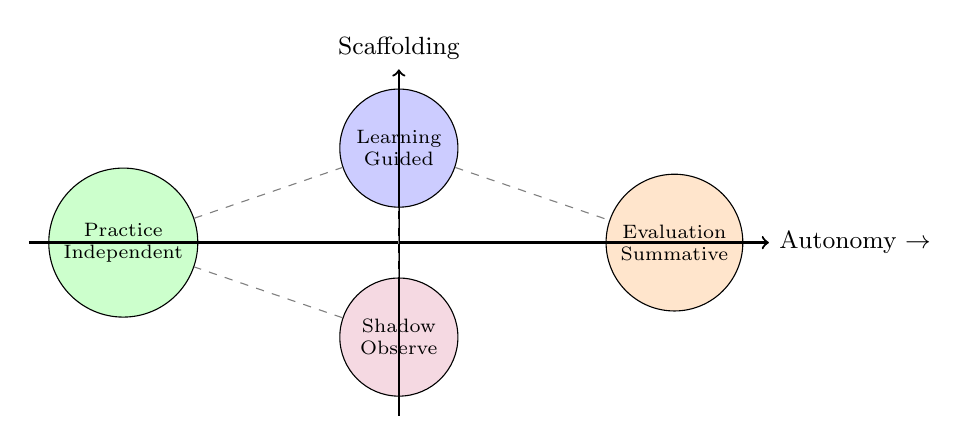
\begin{tikzpicture}[
    mode/.style={circle, draw, minimum size=1.5cm, font=\scriptsize, align=center},
    axis/.style={->, thick}
  ]
    \node[mode, fill=green!20] (p) at (0,0) {Practice\\Independent};
    \node[mode, fill=blue!20] (l) at (3.5,1.2) {Learning\\Guided};
    \node[mode, fill=orange!20] (e) at (7,0) {Evaluation\\Summative};
    \node[mode, fill=purple!15] (s) at (3.5,-1.2) {Shadow\\Observe};
    \draw[axis] (-1.2,0) -- (8.2,0) node[right,font=\small] {Autonomy $\rightarrow$};
    \draw[axis] (3.5,-2.2) -- (3.5,2.2) node[above,font=\small] {Scaffolding};
    \draw[dashed, gray] (p) -- (l);
    \draw[dashed, gray] (l) -- (e);
    \draw[dashed, gray] (s) -- (l);
    \draw[dashed, gray] (s) -- (p);
  \end{tikzpicture}
  \caption{Pedagogical positioning of MedPrep modes along scaffolding vs.\ learner autonomy axes.}
  \label{fig:mode-pedagogy}
\end{figure}


\section{MedPrep AI: Detailed Design}
\subsection{Mode-to-Slug Mapping}
Subscription entitlements reference URL slugs; the backend maps slugs to Prisma \texttt{MedprepMode} enum values (Table~\ref{tab:slug-map}).

\begin{table}[htbp]
  \centering
  \caption{MedPrep slug $\leftrightarrow$ enum mapping (\texttt{medprep-mode-map.ts}).}
  \label{tab:slug-map}
  \begin{tabular}{@{}lll@{}}
    \toprule
    \textbf{UI slug} & \textbf{Prisma enum} & \textbf{Standalone path} \\
    \midrule
    \texttt{let-me-drive} & PRACTICE & \texttt{/practice-mode} \\
    \texttt{qa} & LEARNING & \texttt{/learning-mode} \\
    \texttt{ai-evaluation} & EVALUATION & \texttt{/evaluation} \\
    \texttt{shadow-mode} & SHADOW & \texttt{/shadow-mode} \\
    \bottomrule
  \end{tabular}
\end{table}

\subsection{Encounter State Machine}
Conversation status transitions follow Figure~\ref{fig:state-machine}.

\begin{figure}[htbp]
  \centering
  \begin{tikzpicture}[
    state/.style={rectangle, rounded corners, draw, minimum width=2.2cm, minimum height=0.65cm, font=\scriptsize},
    every path/.style={->, >=stealth}
  ]
    \node[state, fill=green!15] (active) at (0,0) {ACTIVE};
    \node[state, fill=blue!12, right=3.2cm of active] (done) {COMPLETED};
    \node[state, fill=red!10, below=1.2cm of active] (abandon) {ABANDONED};
    \draw (active) -- node[above,font=\tiny]{submit dx/SOAP} (done);
    \draw (active) -- node[left,font=\tiny]{timeout/exit} (abandon);
    \draw[dashed] (abandon) -- node[below,font=\tiny]{resume new} (active);
  \end{tikzpicture}
  \caption{MedPrep conversation state machine.}
  \label{fig:state-machine}
\end{figure}

% Included by methodology — MedPrep encounter sequence
\begin{figure}[htbp]
  \centering
  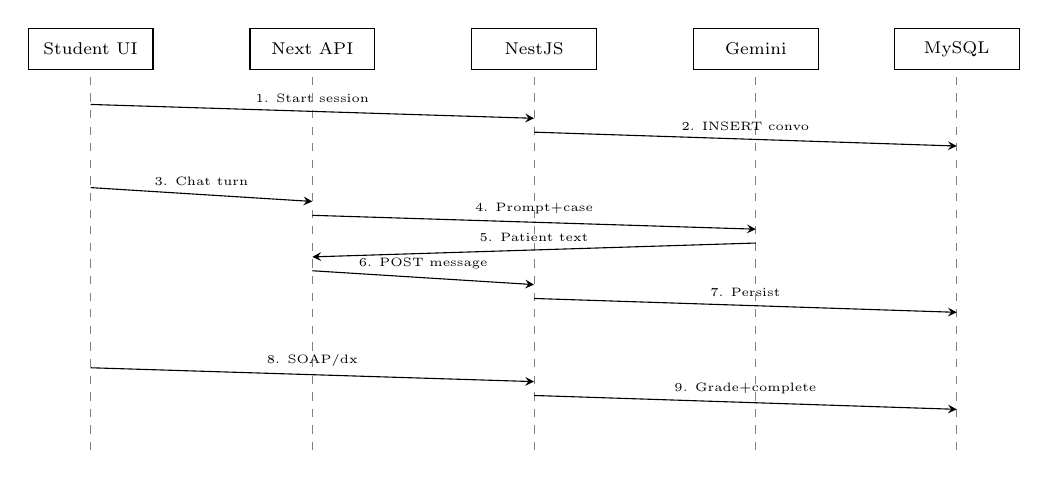
\begin{tikzpicture}[
    scale=0.88,
    transform shape,
    node distance=0.55cm,
    actor/.style={rectangle, draw, minimum width=1.8cm, minimum height=0.6cm, font=\scriptsize},
    msg/.style={->, >=stealth, font=\tiny},
    lifeline/.style={dashed, gray}
  ]
    \node[actor] (stu) at (0,0) {Student UI};
    \node[actor] (next) at (3.2,0) {Next API};
    \node[actor] (nest) at (6.4,0) {NestJS};
    \node[actor] (llm) at (9.6,0) {Gemini};
    \node[actor] (db) at (12.5,0) {MySQL};
    \foreach \x in {0,3.2,6.4,9.6,12.5} {
      \draw[lifeline] (\x,-0.4) -- (\x,-5.8);
    }
    \draw[msg] (0,-0.8) -- node[above] {1. Start session} (6.4,-1.0);
    \draw[msg] (6.4,-1.2) -- node[above] {2. INSERT convo} (12.5,-1.4);
    \draw[msg] (0,-2.0) -- node[above] {3. Chat turn} (3.2,-2.2);
    \draw[msg] (3.2,-2.4) -- node[above] {4. Prompt+case} (9.6,-2.6);
    \draw[msg] (9.6,-2.8) -- node[above] {5. Patient text} (3.2,-3.0);
    \draw[msg] (3.2,-3.2) -- node[above] {6. POST message} (6.4,-3.4);
    \draw[msg] (6.4,-3.6) -- node[above] {7. Persist} (12.5,-3.8);
    \draw[msg] (0,-4.6) -- node[above] {8. SOAP/dx} (6.4,-4.8);
    \draw[msg] (6.4,-5.0) -- node[above] {9. Grade+complete} (12.5,-5.2);
  \end{tikzpicture}
  \caption{Sequence of operations for a single MedPrep encounter turn (simplified).}
  \label{fig:medprep-sequence}
\end{figure}


\subsection{REST API Surface (MedPrep Module)}
Table~\ref{tab:medprep-api} lists principal MedPrep AI endpoints (Swagger-documented).

\begin{table}[htbp]
  \centering
  \caption{Principal MedPrep AI REST endpoints.}
  \label{tab:medprep-api}
  \footnotesize
  \setlength{\tabcolsep}{4pt}
  \renewcommand{\arraystretch}{1.15}
  \begin{tabular}{@{}lP{4.1cm}P{5.6cm}@{}}
    \toprule
    \textbf{Method} & \textbf{Path} & \textbf{Description} \\
    \midrule
    GET & \api{/medprep-ai/modes} & List mode metadata for marketing/UI \\
    POST & \api{/medprep-ai/sessions} & Start or resume ACTIVE session \\
    GET & \api{/medprep-ai/sessions} & List sessions (optional summary mode) \\
    GET & \api{/medprep-ai/sessions/:id} & Full session with messages, SOAP \\
    POST & \api{/medprep-ai/sessions/:id/messages} & Append STUDENT/PATIENT/DOCTOR msg \\
    POST & \api{/medprep-ai/sessions/:id/diagnosis} & Submit diagnosis vs.\ ground truth \\
    PUT & \api{/medprep-ai/sessions/:id/soap} & Upsert SOAP sections \\
    POST & \api{/medprep-ai/sessions/:id/complete} & Mark COMPLETED, set score \\
    PUT & \api{/medprep-ai/hint-sessions} & Upsert Learning hint telemetry \\
    \bottomrule
  \end{tabular}
\end{table}

\subsection{Message Roles and Clinical Semantics}
Three roles are persisted (\texttt{MedprepMessageRole}):
\begin{itemize}
  \item \textbf{STUDENT}: learner questions, exam requests, management plans;
  \item \textbf{PATIENT}: simulated patient speech (LLM-generated, temperature-tuned for realism);
  \item \textbf{DOCTOR}: attending reasoning in Shadow/Learning (may include hidden chain-of-thought summaries stored in metadata).
\end{itemize}
The \texttt{isIntervention} flag marks faculty-style teaching moments in Shadow mode; \texttt{relevanceScore} optionally records automated scoring of student question quality.

\subsection{Hint Session Grading Model}
Learning mode penalizes excessive hints. Let $h_{hi}, h_{med}, h_{lo}$ be hint counts by importance. The platform stores an aggregate \texttt{gradePenalty} computed from weighted hint usage (implementation in frontend learning utilities), enabling faculty to distinguish students who solved cases independently vs.\ those requiring maximal scaffolding.

\subsection{SOAP Documentation Model}
SOAP notes decompose the clinical encounter into four canonical sections (Table~\ref{tab:soap}).

\begin{table}[htbp]
  \centering
  \caption{SOAP sections and AI mirror fields.}
  \label{tab:soap}
  \begin{tabular}{@{}p{2cm}p{5.5cm}p{5.5cm}@{}}
    \toprule
    \textbf{Section} & \textbf{Student field} & \textbf{AI feedback field} \\
    \midrule
    S & \texttt{subjective} & \texttt{aiSubjective} \\
    O & \texttt{objective} & \texttt{aiObjective} \\
    A & \texttt{assessment} & \texttt{aiAssessment} \\
    P & \texttt{plan} & \texttt{aiPlan} \\
    \bottomrule
  \end{tabular}
\end{table}

\subsection{Shadow Mode: Metadata and Caps}
Shadow sessions store large encounter artifacts in \texttt{MedprepConversation.metadata} JSON:
\begin{itemize}
  \item Doctor thought streams and differential diagnosis snapshots;
  \item Ordered investigations with structured test reports;
  \item Intervention Q\&A capped at 48 entries, 4000 characters per field (prevent unbounded JSON);
  \item Replay index for step-through UI.
\end{itemize}
Synchronization logic (\texttt{shadow-medprep-db-sync.ts}) batches updates to Nest after meaningful encounter milestones, balancing realtime UX with database consistency.

\subsection{Case Generation Pipeline}
\texttt{POST /api/cases/generate} invokes Gemini with a JSON schema prompt; on failure, a rule-based fallback generator supplies demo cases. Generated cases set \texttt{isGeneratedCase=true} on conversations, subject to per-mode distinct-case quotas enforced server-side to limit API abuse.

\section{LLM Integration Architecture}
\begin{figure}[htbp]
  \centering
  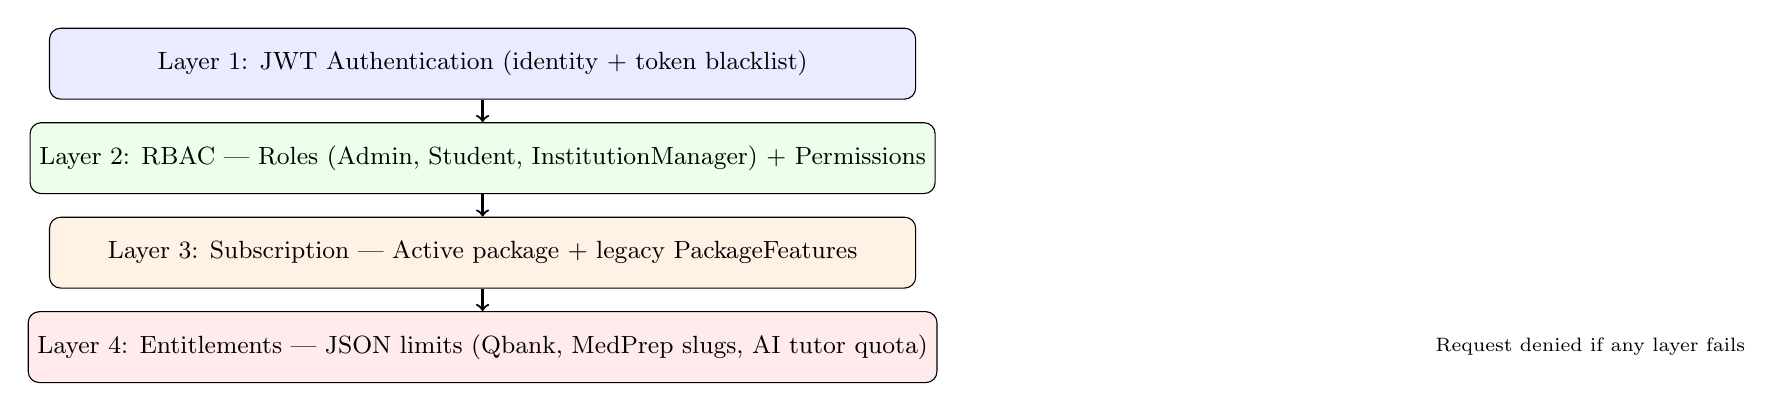
\begin{tikzpicture}[
    layer/.style={rectangle, draw, rounded corners, minimum width=11cm, minimum height=0.9cm, align=center, font=\small},
    arr/.style={->, thick}
  ]
    \node[layer, fill=blue!8] (l1) at (0,3.2) {Layer 1: JWT Authentication (identity + token blacklist)};
    \node[layer, fill=green!8] (l2) at (0,2.0) {Layer 2: RBAC --- Roles (Admin, Student, InstitutionManager) + Permissions};
    \node[layer, fill=orange!10] (l3) at (0,0.8) {Layer 3: Subscription --- Active package + legacy PackageFeatures};
    \node[layer, fill=red!8] (l4) at (0,-0.4) {Layer 4: Entitlements --- JSON limits (Qbank, MedPrep slugs, AI tutor quota)};
    \draw[arr] (l1) -- (l2);
    \draw[arr] (l2) -- (l3);
    \draw[arr] (l3) -- (l4);
    \node[font=\scriptsize, right=6.2cm] at (l4.east) {Request denied if any layer fails};
  \end{tikzpicture}
  \caption{Defense-in-depth access control stack in MedPrepAI.}
  \label{fig:rbac-layers}
\end{figure}


Figure~\ref{fig:llm-arch} shows how LLM calls are distributed (not all traffic passes through Nest---latency-sensitive dialogue uses Next API routes).

\begin{figure}[htbp]
  \centering
  \begin{tikzpicture}[
    box/.style={rectangle, draw, rounded corners, minimum width=2.5cm, minimum height=0.7cm, font=\scriptsize, align=center}
  ]
    \node[box, fill=blue!10] (ui) {React Chat UI};
    \node[box, fill=orange!12, below=1cm of ui] (routes) {Next.js API Routes\\\texttt{/api/learning/*}};
    \node[box, fill=green!10, below left=1cm and 0.2cm of routes] (gem) {Gemini API};
    \node[box, fill=purple!10, below right=1cm and 0.2cm of routes] (nest) {NestJS AiTutor\\MedPrep persist};
    \node[box, fill=gray!10, below=1cm of nest] (sql) {MySQL};
    \draw[->] (ui) -- (routes);
    \draw[->] (routes) -- (gem);
    \draw[->] (ui) -- node[right,font=\tiny]{REST} (nest);
    \draw[->] (nest) -- (sql);
    \draw[->, dashed] (routes) -- node[font=\tiny,above]{optional persist} (nest);
  \end{tikzpicture}
  \caption{LLM call paths: encounter dialogue via Next API; persistence via NestJS.}
  \label{fig:llm-arch}
\end{figure}

\begin{table}[htbp]
  \centering
  \caption{Next.js API routes for clinical LLM orchestration.}
  \label{tab:llm-routes}
  \footnotesize
  \setlength{\tabcolsep}{4pt}
  \renewcommand{\arraystretch}{1.2}
  \begin{tabular}{@{}P{0.38\textwidth}P{0.56\textwidth}@{}}
    \toprule
    \textbf{Route} & \textbf{Function} \\
    \midrule
    \api{/api/learning/patient-response} & Generate patient utterance from case + history \\
    \api{/api/learning/doctor-thought} & Attending reasoning for Shadow/Learning \\
    \api{/api/learning/differential-diagnosis} & Update DDx list with probabilities \\
    \api{/api/learning/ai-supervisor} & Formative hints in Learning mode \\
    \api{/api/learning/generate-prescription} & Shadow prescribing step \\
    \api{/api/cases/generate} & LLM batch case authoring \\
    \api{/api/conversations} & Proxy to Nest session CRUD \\
    \bottomrule
  \end{tabular}
\end{table}

Gemini configuration defaults to \texttt{gemini-2.5-flash} with API keys loaded from \texttt{GOOGLE\_API\_KEY} or \texttt{GEMINI\_API\_KEY}. The helper \texttt{hydrateGeminiApiKeyFromBackendEnv} allows frontend-only dev setups to borrow backend secrets securely during local development.

\section{Learning Management System: Deep Dive}
\begin{figure}[htbp]
  \centering
  \begin{tikzpicture}[
    entity/.style={rectangle, draw, minimum width=2.1cm, minimum height=0.65cm, font=\scriptsize, align=center},
    rel/.style={->, >=stealth}
  ]
    \node[entity] (prod) {Product};
    \node[entity, right=1.4cm of prod] (sec) {Section};
    \node[entity, right=1.4cm of sec] (ch) {Chapter};
    \node[entity, below=1.1cm of ch] (top) {Topic};
    \node[entity, left=1.4cm of top] (q) {Question};
    \node[entity, left=1.4cm of q] (qc) {QuestionChoice};
    \node[entity, below=1.1cm of q] (qp) {QuestionPaper};
    \node[entity, left=1.4cm of qp] (qpq) {QPQuestion};
    \draw[rel] (prod) -- node[above,font=\tiny]{1:N} (sec);
    \draw[rel] (sec) -- node[above,font=\tiny]{1:N} (ch);
    \draw[rel] (ch) -- node[right,font=\tiny]{1:N} (top);
    \draw[rel] (top) -- node[above,font=\tiny]{1:N} (q);
    \draw[rel] (q) -- node[above,font=\tiny]{1:N} (qc);
    \draw[rel] (qp) -- node[above,font=\tiny]{1:N} (qpq);
    \draw[rel] (q) -- node[right,font=\tiny]{N:M} (qpq);
  \end{tikzpicture}
  \caption{Core LMS content hierarchy and assessment linkage.}
  \label{fig:lms-er}
\end{figure}


\subsection{Question Model}
Each \texttt{Question} record includes difficulty, points, stem HTML, explanation blocks, tags, and system/category associations. \texttt{QuestionChoice} rows store labeled options (A--E) with per-choice explanation fragments for rich remediation---critical for USMLE-style learning where wrong-answer teaching is as valuable as correct-answer recall.

\subsection{Test Session Workflow}
Figure~\ref{fig:test-flow} outlines the student test lifecycle.
% Test workflow — tabular layout (avoids TikZ node overlap on Overleaf)
\begin{figure}[H]
  \centering
  \vspace{0.3em}
  \resizebox{\textwidth}{!}{%
  \begin{tabular}{@{}c@{$\rightarrow$}c@{$\rightarrow$}c@{$\rightarrow$}c@{$\rightarrow$}c@{$\rightarrow$}c@{}}
    \fbox{\parbox{1.45cm}{\centering\scriptsize Create\\paper}} &
    \fbox{\parbox{1.45cm}{\centering\scriptsize Select\\questions}} &
    \fbox{\parbox{1.45cm}{\centering\scriptsize Start\\session}} &
    \fbox{\parbox{1.45cm}{\centering\scriptsize Answer\\items}} &
    \fbox{\parbox{1.45cm}{\centering\scriptsize Submit}} &
    \fbox{\parbox{1.55cm}{\centering\scriptsize Results\\analytics}}
  \end{tabular}%
  }
  \vspace{0.3em}
  \caption{Student QBank test session workflow.}
  \label{fig:test-flow}
\end{figure}


\subsection{DOCX and Markdown Ingestion}
The DOCX pipeline executes in stages:
\begin{enumerate}
  \item Upload document to admin endpoint (\texttt{convert-docx.dto});
  \item Extract paragraphs, tables, and embedded images;
  \item Map structural patterns (stem, choices A--E, explanation blocks) to normalized JSON;
  \item Optional LLM pass resolves ambiguous formatting;
  \item Validate media URLs; persist via \texttt{QuestionsService}.
\end{enumerate}
This pipeline is documented in \texttt{DOCX\_LLM\_WORKFLOW.md} and enables bulk import of publisher-style item banks.

\subsection{Mock Exams and Self-Assessment}
Mock exam module enforces timed blocks and locked navigation similar to national exams. Subscription feature ``Self Assessment'' may include monthly quotas tracked via \texttt{EntitlementUsage} with \texttt{NUMBER\_LIMIT} type---demonstrating migration from legacy boolean \texttt{PackageFeatures} to parameterized entitlements.

\section{Access Control and Entitlements}
\subsection{Access Control Matrix}
Table~\ref{tab:access-matrix} reproduces the platform RBAC/subscription matrix from implementation docs.

\begin{table}[htbp]
  \centering
  \caption{Access control matrix (selected resources).}
  \label{tab:access-matrix}
  \footnotesize
  \begin{tabular}{@{}lccccc@{}}
    \toprule
    \textbf{Resource} & \textbf{Admin} & \textbf{Stu. (no sub)} & \textbf{Basic} & \textbf{Premium} & \textbf{Inst.\ Mgr.} \\
    \midrule
    Dashboard & Full & Limited & Full & Full & Full \\
    Qbank & All & --- & Limited & All & All \\
    Self Assessment & All & --- & --- & 1/mo & All \\
    Create Question & Yes & No & No & No & No \\
    Study Planner & Yes & No & No & Yes & Yes \\
    MedPrep Shadow & Yes & No & No & Entitled & Yes \\
    Faculty compare & Yes & No & No & No & Yes \\
    \bottomrule
  \end{tabular}
\end{table}

\subsection{Entitlement Type System}
The modern entitlement layer supports types in Table~\ref{tab:entitlement-types}.

\begin{table}[htbp]
  \centering
  \caption{EntitlementDefinition types (\texttt{subscription.schema.prisma}).}
  \label{tab:entitlement-types}
  \begin{tabular}{@{}lp{9.8cm}@{}}
    \toprule
    \textbf{Type} & \textbf{Semantics} \\
    \midrule
    BOOLEAN & Feature on/off (e.g., Qbank access) \\
    SET & Allow-list of slugs (e.g., MedPrep modes) \\
    NUMBER\_LIMIT & Quota per billing period (e.g., AI tutor messages) \\
    JSON\_CONSTRAINTS & Complex rules in \texttt{valueJson} \\
    \bottomrule
  \end{tabular}
\end{table}

\subsection{Guard Composition}
NestJS controllers compose guards declaratively:
\begin{verbatim}
@UseGuards(JwtAuthGuard, FeatureGuard)
@RequiredFeatures('Qbank Access')
\end{verbatim}
Combined requirements (role + subscription + feature) use \texttt{CombinedAccessGuard} on sensitive admin routes. This pattern implements \emph{policy-as-code}, auditable in version control.

\section{Faculty and Institution Modules}
\subsection{Faculty Analytics Queries}
\texttt{FacultyService} aggregates per-student:
\begin{itemize}
  \item Count of completed MedPrep conversations (7-day window);
  \item Average session score where available;
  \item Assignment completion percentage.
\end{itemize}
These metrics power \texttt{/faculty/compare} visualizations for identifying at-risk students before high-stakes exams.

\subsection{Assignment Synchronization}
When a MedPrep session transitions to COMPLETED, an asynchronous hook invokes \texttt{StudentInstitutionService.syncAssignmentFromMedprepSession} so curricular assignments reflect student progress without manual faculty clicks.

\subsection{Institution Domain Linking}
Students registering with institutional email domains auto-associate to \texttt{InstitutionMember} records, unlocking institution-published cases and faculty messaging channels (\texttt{ChatRoomType.FACULTY\_STUDENT}).

\section{Community, Realtime, and Engagement}
\subsection{Discussion and Study Groups}
Discussion threads support curricular Q\&A; study groups add owned communities with posts---social presence increases retention in longitudinal subscriptions.

\subsection{Achievements and Points}
\texttt{AchievementsService} evaluates rules (e.g., \texttt{MEDPREP\_CONVERSATIONS}, \texttt{MEDPREP\_CASE\_LOAD}) against activity counters, awarding badges and points logged in \texttt{UserPoints}. Gamification is optional pedagogically but valuable for student motivation.

\subsection{Chat and Notifications}
Chat schema includes room types, participants, reactions, read receipts. Notifications support preferences per channel (email/in-app). \texttt{RealtimeModule} pushes Socket.IO events for low-latency message delivery.

\section{Payments and Subscription Lifecycle}
Stripe webhooks update subscription status; failed payments downgrade entitlements on next API call via \texttt{getUserActiveFeatures}. Table~\ref{tab:payment-entities} lists payment schema entities.

\begin{table}[htbp]
  \centering
  \caption{Payment module entities.}
  \label{tab:payment-entities}
  \small
  \begin{tabular}{@{}lp{9.2cm}@{}}
    \toprule
    \textbf{Model} & \textbf{Role} \\
    \midrule
    PaymentMethod & Stored cards via Stripe customer \\
    Payment & Transaction history \\
    Wallet & Internal credit balance \\
    PromoCode & Discount campaigns \\
    Invoice & Billing records for UI history page \\
    \bottomrule
  \end{tabular}
\end{table}

\section{Deployment and Operations}
\begin{figure}[htbp]
  \centering
  \begin{tikzpicture}[
    box/.style={rectangle, draw, rounded corners, minimum width=2.4cm, minimum height=0.7cm, align=center, font=\scriptsize}
  ]
    \node[box, fill=gray!12] (user) {Browser / Student};
    \node[box, fill=cyan!15, below=1.1cm of user] (nginx) {Nginx (TLS, reverse proxy)};
    \node[box, fill=blue!10, below left=0.9cm and 0.3cm of nginx] (fe) {Next.js :3001};
    \node[box, fill=blue!10, below right=0.9cm and 0.3cm of nginx] (be) {NestJS API};
    \node[box, fill=yellow!15, below=1.0cm of be] (db) {MySQL};
    \node[box, fill=green!12, right=1.6cm of be] (ext) {Stripe / Gemini APIs};
    \draw[->] (user) -- (nginx);
    \draw[->] (nginx) -- (fe);
    \draw[->] (nginx) -- node[font=\tiny,right]{/api} (be);
    \draw[->] (be) -- (db);
    \draw[->] (be) -- (ext);
    \draw[->, dashed] (fe) -- node[font=\tiny,above]{SSR + API routes} (be);
  \end{tikzpicture}
  \caption{Production deployment topology (clinical-lab on cloud VM with PM2).}
  \label{fig:deployment}
\end{figure}


\subsection{Build and Release Process}
Production release steps:
\begin{enumerate}
  \item Run unit tests (\texttt{jest}) on backend; lint frontend;
  \item \texttt{npm run build} for Nest and Next;
  \item Rsync to EC2 host excluding \texttt{node\_modules};
  \item \texttt{prisma migrate deploy}; \texttt{pm2 restart all};
  \item Smoke test: login, start MedPrep session, answer one QBank question.
\end{enumerate}

\subsection{Environment Configuration}
Secrets never ship in git; \texttt{.env} on server holds database URL, JWT secret, Gemini key, Stripe keys. Nginx routes \texttt{/api} to Nest and static/SSR to Next on port 3001.

\subsection{Demo Seed Dataset}
\texttt{seed-demo-full.ts} creates labeled \texttt{[Demo]} entities across all MedPrep modes, discussions, study groups, achievements, and feedback---enabling reproducible thesis demonstrations without manual data entry.

\section{Data Model Summary}
Table~\ref{tab:schema-files} enumerates all Prisma schema modules.

\begin{table}[htbp]
  \centering
  \caption{Prisma schema files and primary entities.}
  \label{tab:schema-files}
  \footnotesize
  \begin{tabular}{@{}p{3.8cm}p{9.4cm}@{}}
    \toprule
    \textbf{File} & \textbf{Primary entities} \\
    \midrule
    base.schema & User, Role, Permission, Institution, AuditLog \\
    product.schema & Product, ProductTag, ProductSubtype \\
    content.schema & Section, Chapter, Topic, Question, QuestionChoice \\
    assessment.schema & QuestionPaper, QuestionPaperQuestion \\
    subscription.schema & Package, Subscription, Entitlement* \\
    medprep.schema & MedprepConversation, Message, SOAP, Hints \\
    faculty.schema & FacultyProfile, Assignments \\
    student.schema & Activity events, assignment progress \\
    chat.schema & ChatRoom, ChatMessage \\
    notification.schema & Notification, preferences \\
    ai-tutor.schema & AiTutorConversation, messages \\
    mock-exam.schema & MockExam, attempts \\
    achievement.schema & Achievement, UserAchievement \\
    discussion.schema & Discussion, Reply \\
    study-group.schema & StudyGroup, Member, Post \\
    feedback.schema & FeedbackTicket \\
    question-report.schema & QuestionReport \\
    goal.schema & Goal, milestones \\
    payment.schema & Payment, Wallet, Stripe linkage \\
    \bottomrule
  \end{tabular}
\end{table}

\section{Testing and Quality Assurance}
Quality practices include:
\begin{itemize}
  \item \texttt{medprep-ai.service.spec.ts} unit tests for session rules;
  \item \texttt{logout.test.ts} for token blacklist;
  \item Manual QA scripts via demo seed and db-viewer;
  \item Swagger UI for contract verification during frontend integration.
\end{itemize}

Future work should add E2E tests (Playwright) for critical encounter paths; capstone timeline prioritized feature delivery.


\section{Implementation Summary}
MedPrepAI comprises $>$25 NestJS feature modules and hundreds of frontend components. TypeScript end-to-end ensures DTO validation (\texttt{class-validator}) aligns with UI types. Swagger documents REST contracts for reproducible integration testing. The clinical-lab repository thus represents a capstone-scale software product, not a prototype limited to a single AI chat screen.
